\documentclass[12pt,a4paper]{scrartcl}
\usepackage[utf8]{inputenc}
\usepackage[english, russian]{babel}
\usepackage{indentfirst}
\usepackage{misccorr}
\usepackage[dvipdfmx]{graphicx}
\usepackage{amsmath}
\usepackage{multirow}
\usepackage{pgfplots}
\usepackage{parskip}
\usepackage[top=1cm, bottom=1cm, left=1cm, right=1cm]{geometry}
\pgfplotsset{compat=1.9}

\begin{document}
	\graphicspath{{py/}}
	
	\newcommand{\ms}{\mathstrut}
	\newcommand{\msp}{\hspace{0.5cm}}
	\newcommand{\al}{\alpha}
	\newcommand{\dg}{^\circ}
	\newcommand{\dif}{\mathrm{d}}
	\newcommand{\qd}[2]{^{\frac{#1}{#2}}}
	\newcommand{\qdm}[2]{^{-\frac{#1}{#2}}}
	\newcommand{\lm}[2]{\underset{#1 \rightarrow #2}{\lim}}
	\newcommand{\sfrac}[2]{\dfrac{\strut #1}{\strut #2}}
	\newcommand{\equal}[1]{\overset{(#1)}{=}}
	\newcommand{\linevdots}{\ \raisebox{-.08\height}{\vdots}\ }
	\newcommand{\linecvdots}{\ \raisebox{-.08\height}{\vdots}\hspace{-0.13cm}\raisebox{.15\height}{\cancel{\phantom{a}}\hspace{0.06cm}}}
	\newcommand{\combox}[1]{\ms \msp \msp \begin{minipage}{0.95\linewidth}
			#1
	\end{minipage}}
	
	\newtheorem{pr}{Задача}
	\newtheorem{ex}{Пример}
	\newtheorem{dfn}{Def}
	\newtheorem{theorem}{Th}
	
	\newenvironment{slv}{\ms \msp \textit{Решение:}}{}
	\newenvironment{proof}{\ms \msp \textit{Доказательство: }}{\hfill $\square$}
	
	\begin{titlepage}
		
		\vspace*{\fill}
		
		\begin{center}
			
\includegraphics[scale=0.8]{MIPT.png}
			\\[0.7cm]\Huge Московский Физико-Технический Институт\\(национальный исследовательский университет)
			\\[2cm]\LARGE Отчет по эксперименту
			\\[0.5cm]\noindent\rule{\textwidth}{1pt}
			\\\Huge\textbf{Эффект Холла в металлах}
			\\[-0.5cm]\noindent\rule{\textwidth}{1pt}
		\end{center}
		
		\begin{flushleft}
			\textit{Работа №3.3.5; дата: 21.10.22}\hfill\textit{Семестр: 3}
		\end{flushleft}
		
		\vspace*{\fill}
		
		\begin{flushleft}
			Выполнил: \hspace{\fill} Группа:
			\\Кошелев Александр \hspace{\fill} Б05-105
		\end{flushleft}
	\end{titlepage}
	
	%Страница 2
	
	\begin{flushleft}
		\footnotesize{Эффект Холла в металлах} \hspace{\fill} \footnotesize{2}
		\\[-0.3cm]\noindent\rule{\textwidth}{0.3pt}
	\end{flushleft}
	
	\section{Аннотация}
	
	\textbf{Цель работы: }
	
	Измерение подвижности и концентрации носителей заряда в металлах.
	
	\textbf{Схема установки:}
	\begin{center}
		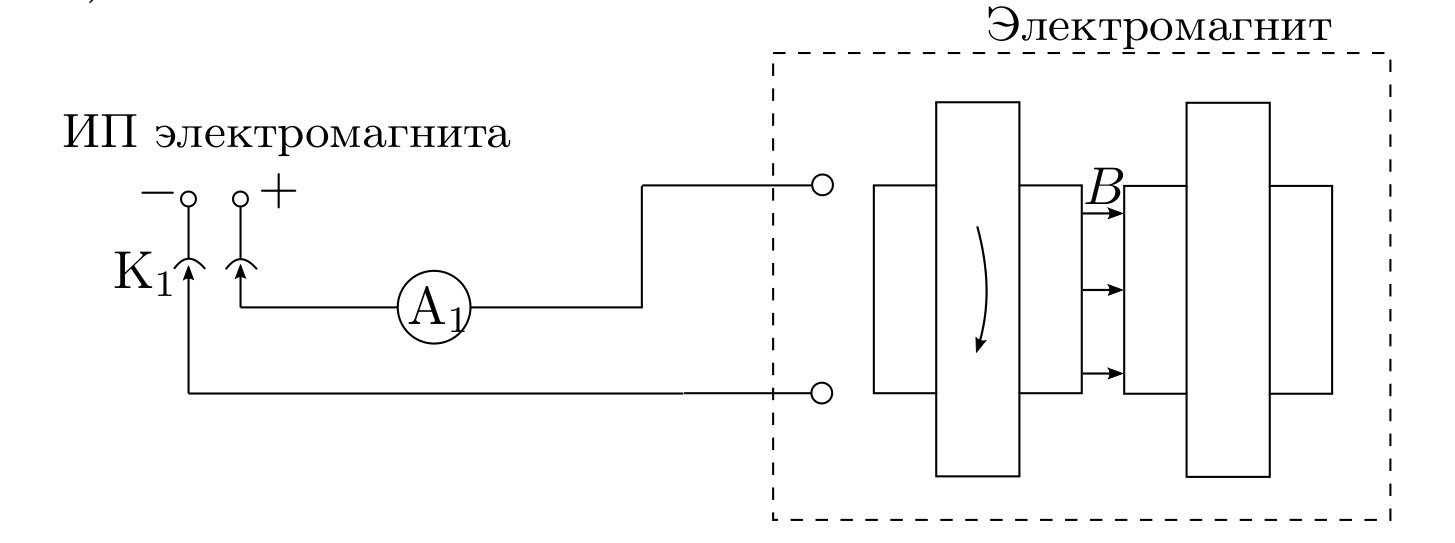
\includegraphics[scale=0.25]{PIC_1.png}
		\\\textbf{Рис. 1:} Схема установки
	\end{center}	

	\begin{center}
		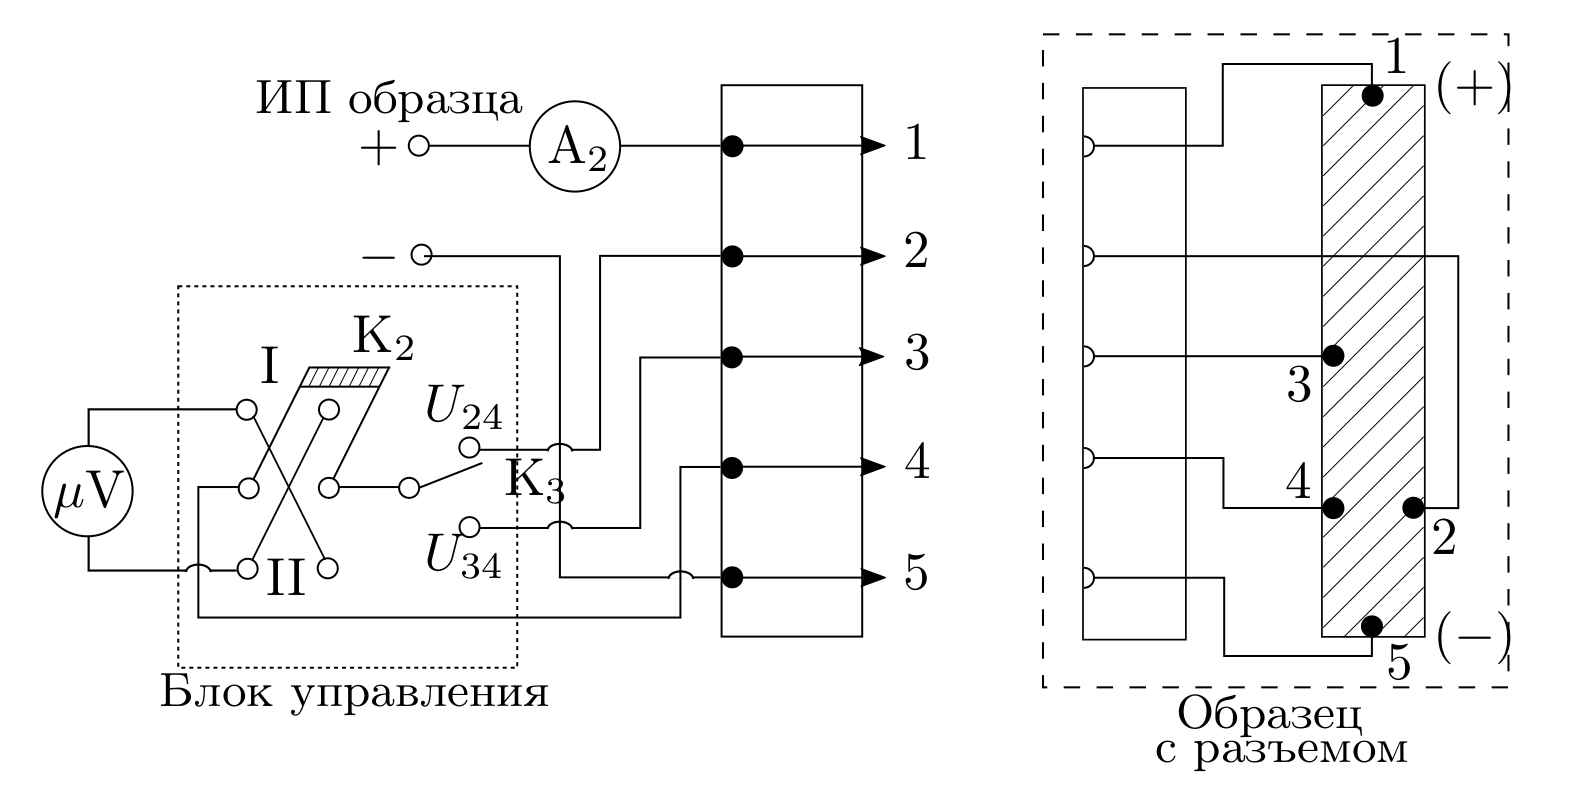
\includegraphics[scale=0.25]{PIC_2.png}
		\\\textbf{Рис. 2:} Схема установки
	\end{center}
		
	В зазоре электромагнита (Рис. 1) создаётся постоянное магнитное поле, величину которого можно менять с помощью источника питания электромагнита. Разъём $K1$ позволяет менять направление тока в обмотках электромагнита. Ток питания электромагнита измеряется амперметром $A1$.
	
	Градуировка электромагнита (связь тока с индукцией поля) проводится при помощи цифрового магнитометра.
	
	Металлические образцы в форме тонких пластинок, смонтированные в специальных держателях, подключаются к блоку питания через разъём (Рис. 2). Ток через образец регулируется реостатом $R2$ и измеряется
	амперметром $A2$.
	
	Для измерений ЭДС Холла используется микровольтметр, в котором высокая чувствительность по напряжению сочетается с малой величиной тока, потребляемого измерительной схемой.
	
	В образце с током, помещённом в зазор электромагнита, между контактами 2 и 4 возникает холловская разность потенциалов $U_\perp$, которая измеряется с помощью микровольтметра, если переключатель $K3$ подключён к точке 2 образца. При подключении $K3$ к точке 3 микровольтметр измеряет омическое падение напряжения $U_{34}$, вызванное током через образец. При нейтральном положении ключа входная цепь микровольтметра разомкнута.	

	\newpage

	%Страница 3

	\begin{flushleft}
		\footnotesize{Эффект Холла в металлах} \hspace{\fill} \footnotesize{3}
		\\[-0.3cm]\noindent\rule{\textwidth}{0.3pt}
	\end{flushleft}		
		
	Ключ $K2$ позволяет менять полярность напряжения, поступающего на вход микровольтметра.	
		
	Контакты 2 и 4 вследствие неточности подпайки могут лежать не на одной эквипотенциали. Тогда напряжение между ними связано не только с эффектом Холла, но и с омическим падением напряжения вдоль пластинки.
	
	Можно исключить влияние омического падения напряжения, если при каждом значении тока через образец измерять на­пряжение между точками 3 и 4 в отсутствие магнитного поля. При фиксированном токе через образец это дополнительное к ЭДС Холла напряжение $U_0$ остаётся неизменным. От него следует отсчитывать величину ЭДС Холла:	$U_\perp = U_{24} - U_0$.
	
	Проводимость образцов можно рассчитать по очевидной формуле:
	
	$$\sigma = \sfrac{Il_{34}}{U_{34}al}$$
		
	\textbf{В работе используются:}
	
	Электромагнит с источником питания, источник постоянного тока, микровольтметр, амперметры, цифровой магнитометр, образцы из меди, серебра и цинка.
	
	\section{Теоретические сведения}
	
	В работе изучаются особенности проводимости металлов в геометрии мостика Холла. Ток пропускается по плоской прямоугольной металлической пластинке, помещённой в перпендикулярное пластинке магнитное поле. Измеряется разность потенциалов между краями пластинки в по­перечном к току направлении. По измерениям определяется константа Холла, тип проводимости (электронный или дырочный) и вычисляется концентрация основных носителей заряда.
	
	\begin{center}
		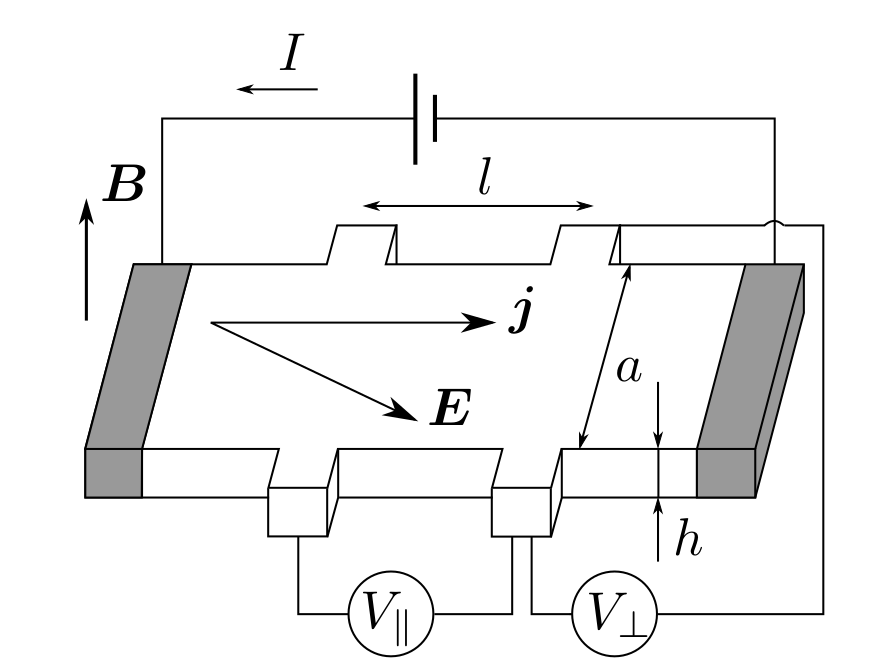
\includegraphics[scale=0.25]{PIC_3.png}
		\\\textbf{Рис. 3:} Схема мостика Холла
	\end{center}
	
	В данной схеме ток вынуждают течь по оси $x$ вдоль плоской пластинки (ширина пластинки $a$, толщина $h$,
	длина $l$). Сила Лоренца, действующая со стороны перпендикулярного пластинке магнитного поля, «прибивает» носители заряда к краям образца, что создаёт холловское электрическое поле, компенсирующее эту	силу. 
	
	Запишем силу Лоренца, действующую на электрон:
	
	$$\vec{F_l} = -e\vec{E} - e\left[\vec{\overline{v}} \times \vec{B}\right] \Rightarrow F_{l, z} = -e E_z + e \overline{v}_x B_y$$
	
	\newpage
	
	%Страница 4
	
	\begin{flushleft}
		\footnotesize{Эффект Холла в металлах} \hspace{\fill} \footnotesize{4}
		\\[-0.3cm]\noindent\rule{\textwidth}{0.3pt}
	\end{flushleft}	
	
	В установившемся режиме $F_{l, z} = 0$, потому:
	
	$$E_z = \overline{v} B$$
	
	При этом величина холловской ЭДС:
	
	$$U_\perp = E_z a = \overline{v} B a$$
	
	С учетом $I = en\overline{v}ah$:
	
	$$U_{\perp} = \sfrac{IB}{neh} = R_x\sfrac{IB}{h}$$
	
	Где $R_x$ -- постоянная Холла.
	
	\section{Ход работы}
	
	\paragraph{Градуировка электромагнита} \hfill
	
	Приведем в таблице градуировку и рассчитаем магнитный коэффициент:
	
	\begin{center}
		\begin{tabular}{|c|c|}
			\hline
			$I_a$, A & $B$, T
			\\\hline
			0.00 $\pm$ 0.00 & 0.000 $\pm$ 0.000
			\\\hline
			0.20 $\pm$ 0.01 & 0.230 $\pm$ 0.010
			\\\hline
			0.35 $\pm$ 0.01 & 0.400 $\pm$ 0.020
			\\\hline
			0.50 $\pm$ 0.01 & 0.580 $\pm$ 0.030
			\\\hline
			0.65 $\pm$ 0.01 & 0.780 $\pm$ 0.040
			\\\hline
			0.80 $\pm$ 0.01 & 0.930 $\pm$ 0.050
			\\\hline
			0.96 $\pm$ 0.01 & 1.050 $\pm$ 0.055
			\\\hline
		\end{tabular}
		\\\textbf{Табл. 1:} Градуировка электромагнита
	\end{center}
	
	\begin{center}
		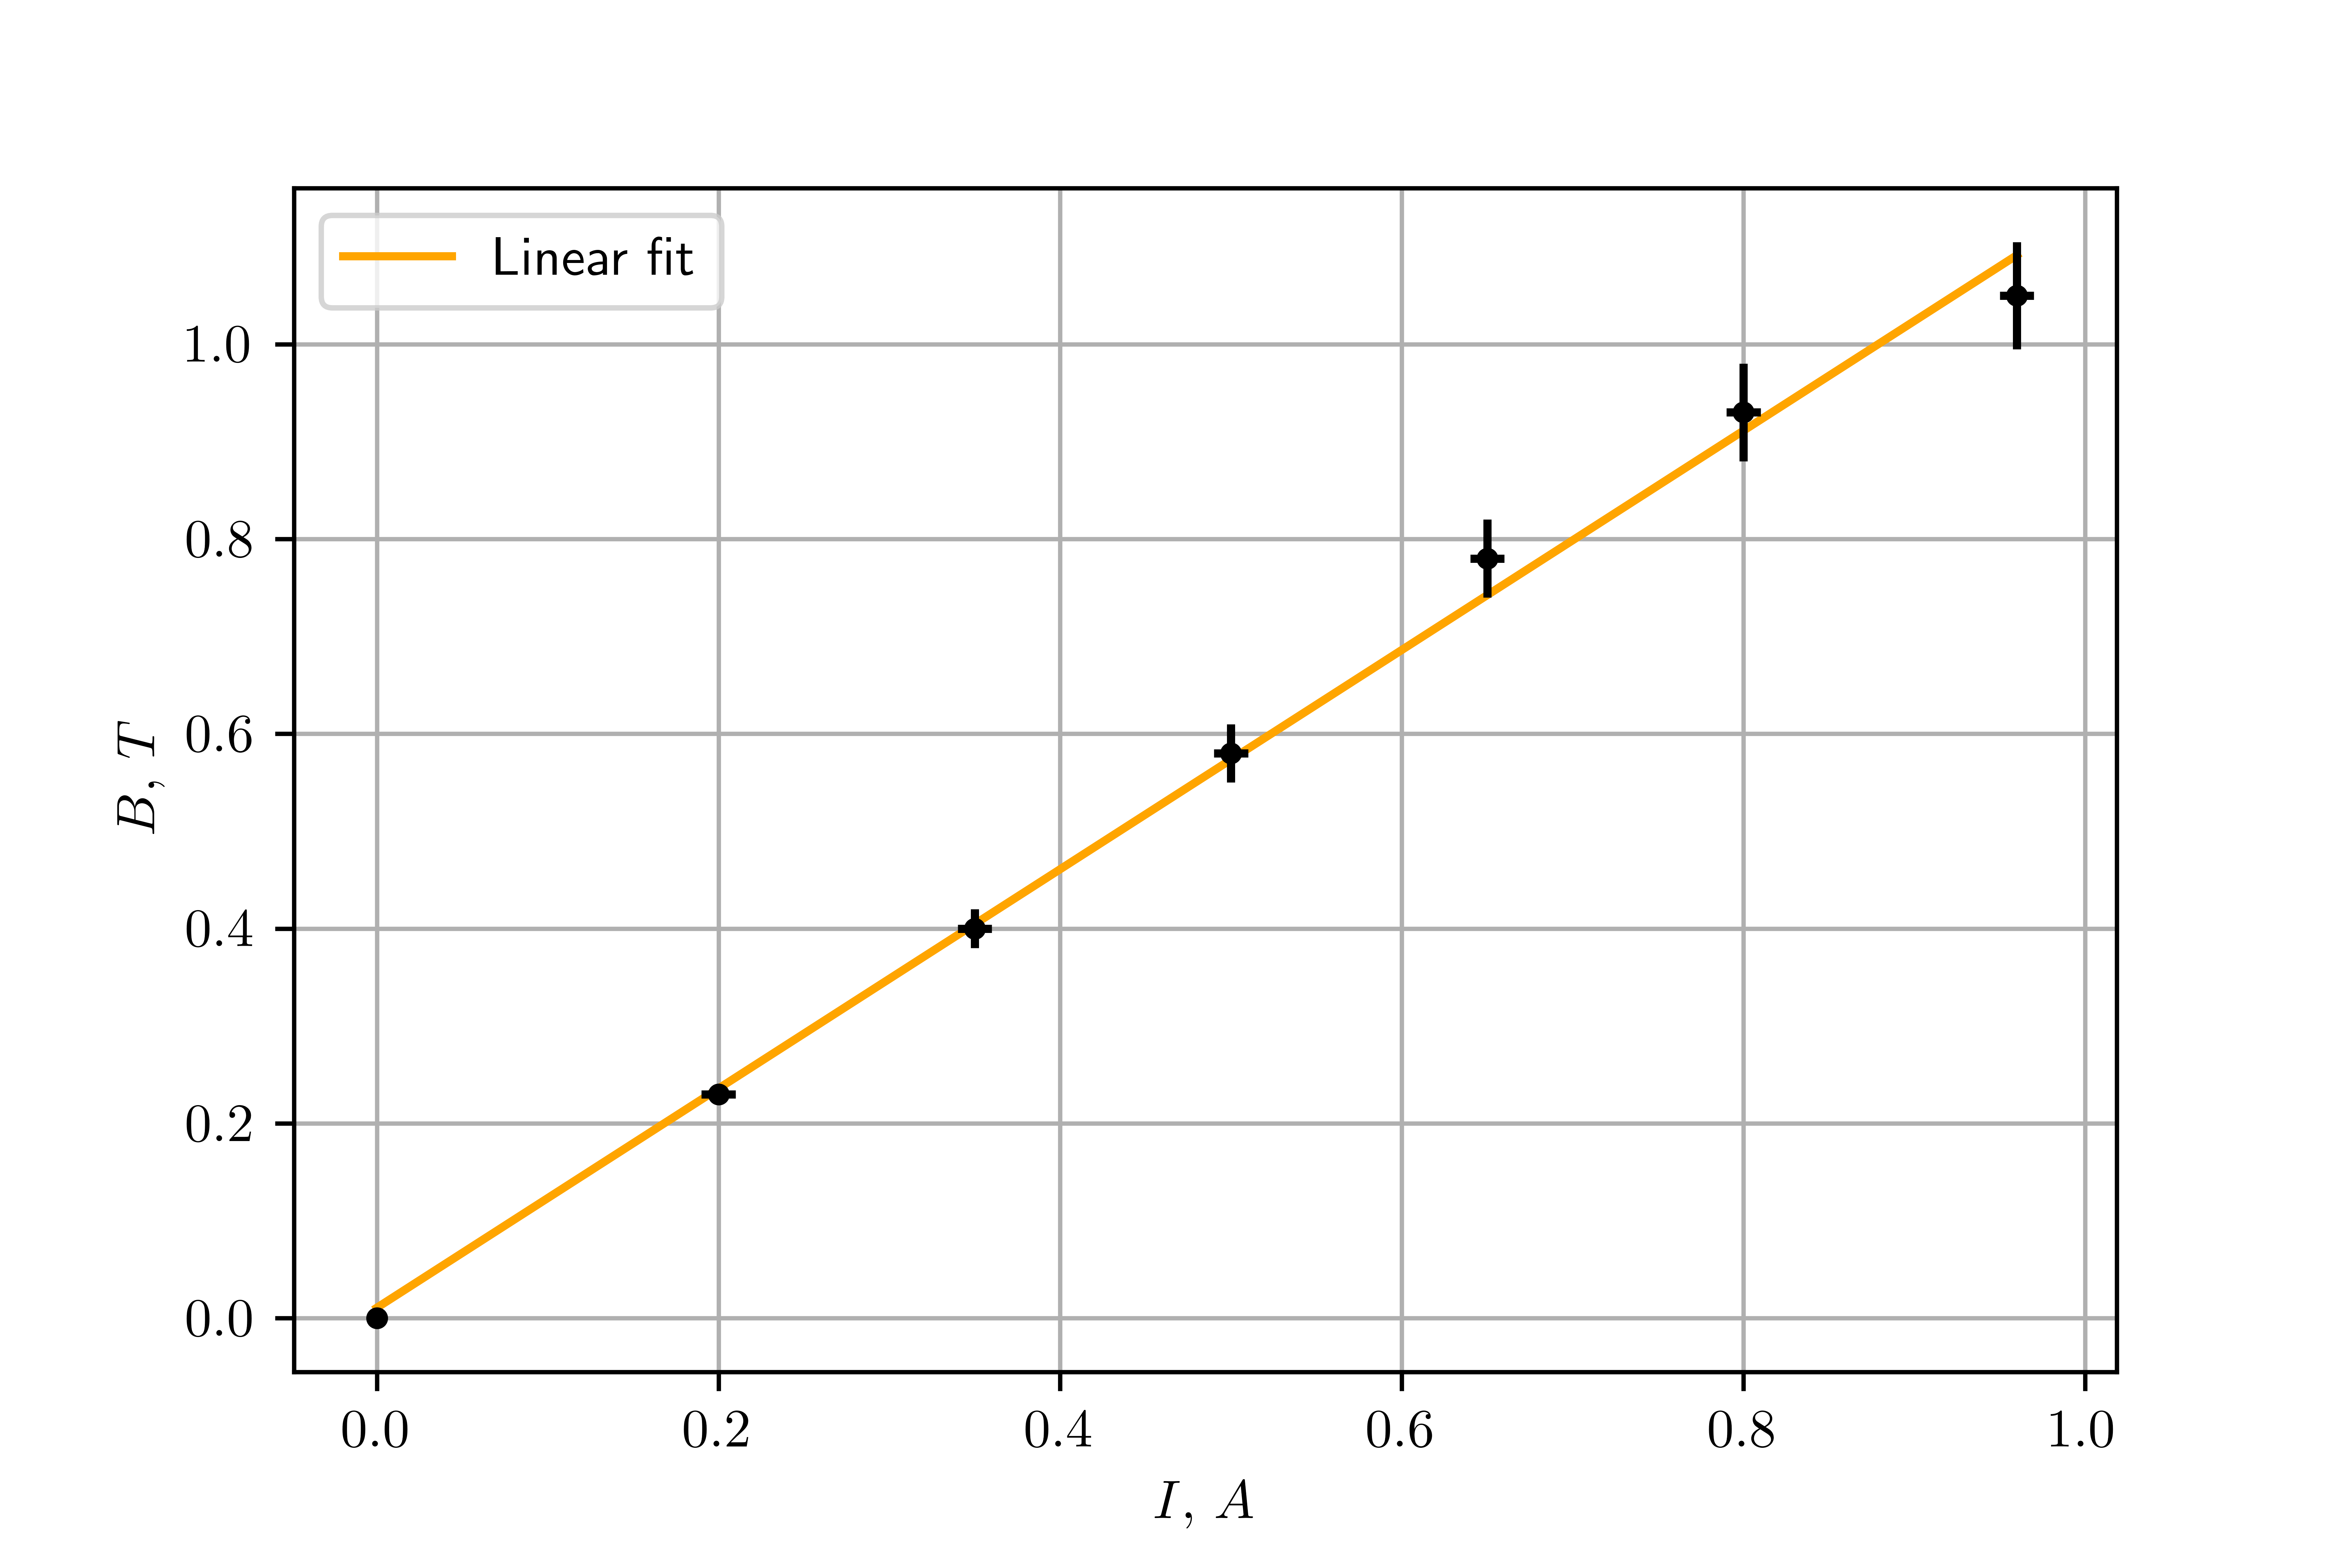
\includegraphics[scale=0.7]{PIC_4.png}
		\\\textbf{Рис. 4:} График зависимости $B(I)$
	\end{center}

	Методом линейной аппроксимации $B = kI + b$ получаем:
	
	$$k = (1.126 \pm 0.033)\, \text{T}/\text{A} \ \ \ \ \ \ \ \ b = (0.011 \pm 0.019)$$
	
	\newpage
	
	%Страница 5
	
	\begin{flushleft}
		\footnotesize{Эффект Холла в металлах} \hspace{\fill} \footnotesize{5}
		\\[-0.3cm]\noindent\rule{\textwidth}{0.3pt}
	\end{flushleft}	
	
	\paragraph{Изучение образца из меди} \hfill
	
	Вначале по направлению ЭДС Холла определяем знак носителей проводимости -- +.
	
	Теперь приведем таблицу измерений:
	
	\begin{center}
		\begin{tabular}{|c|c|c|c|}
			\hline
			\multicolumn{2}{|c|}{$I = (0.4 \pm 0.1)$ A} & \multicolumn{2}{|c|}{$U_0 = (2.0 \pm 0.5)$ un}
			\\\hline
			$I_m$, A & $B$, T & $U_{24}$, un & $U_\perp$, nV
			\\\hline
			$0.20 \pm 0.01$ & $0.236 \pm 0.026$ & $3.0 \pm 0.5$ & $40 \pm 40$
			\\\hline
			$0.39 \pm 0.01$ & $0.450 \pm 0.032$ & $5.0 \pm 0.5$ & $120 \pm 40$
			\\\hline
			$0.60 \pm 0.01$ & $0.687 \pm 0.039$ & $7.0 \pm 0.5$ & $200 \pm 40$
			\\\hline
			$0.80 \pm 0.01$ & $0.912 \pm 0.045$ & $9.0 \pm 0.5$ & $280 \pm 40$
			\\\hline
			$1.01 \pm 0.01$ & $1.148 \pm 0.052$ & $10.0 \pm 0.5$ & $320 \pm 40$
			\\\hline
			$1.20 \pm 0.01$ & $1.362 \pm 0.059$ & $11.0 \pm 0.5$ & $360 \pm 40$
			\\\hline
			\multicolumn{2}{|c|}{$I = (0.6 \pm 0.1)$ A} & \multicolumn{2}{|c|}{$U_0 = (3.0 \pm 0.5)$ un}
			\\\hline
			$I_m$, A & $B$, T & $U_{24}$, un & $U_\perp$, nV
			\\\hline
			$0.20 \pm 0.01$ & $0.236 \pm 0.026$ & $5.0 \pm 0.5$ & $80 \pm 40$
			\\\hline
			$0.40 \pm 0.01$ & $0.461 \pm 0.032$ & $9.0 \pm 0.5$ & $240 \pm 40$
			\\\hline
			$0.60 \pm 0.01$ & $0.687 \pm 0.039$ & $13.0 \pm 0.5$ & $400 \pm 40$
			\\\hline
			$0.80 \pm 0.01$ & $0.912 \pm 0.045$ & $15.0 \pm 0.5$ & $480 \pm 40$
			\\\hline
			$1.00 \pm 0.01$ & $1.137 \pm 0.052$ & $17.0 \pm 0.5$ & $560 \pm 40$
			\\\hline
			$1.20 \pm 0.01$ & $1.362 \pm 0.059$ & $19.0 \pm 0.5$ & $640 \pm 40$
			\\\hline
			\multicolumn{2}{|c|}{$I = (0.8 \pm 0.1)$ A} & \multicolumn{2}{|c|}{$U_0 = (4.0 \pm 0.5)$ un}
			\\\hline
			$I_m$, A & $B$, T & $U_{24}$, un & $U_\perp$, nV
			\\\hline
			$0.20 \pm 0.01$ & $0.236 \pm 0.026$ & $8.0 \pm 0.5$ & $160 \pm 40$
			\\\hline
			$0.40 \pm 0.01$ & $0.461 \pm 0.032$ & $12.0 \pm 0.5$ & $280 \pm 40$
			\\\hline
			$0.60 \pm 0.01$ & $0.687 \pm 0.039$ & $17.0 \pm 0.5$ & $520 \pm 40$
			\\\hline
			$0.80 \pm 0.01$ & $0.912 \pm 0.045$ & $20.0 \pm 0.5$ & $640 \pm 40$
			\\\hline
			$1.00 \pm 0.01$ & $1.137 \pm 0.052$ & $24.0 \pm 0.5$ & $800 \pm 40$
			\\\hline
			$1.20 \pm 0.01$ & $1.362 \pm 0.059$ & $27.0 \pm 0.5$ & $920 \pm 40$
			\\\hline
			\multicolumn{2}{|c|}{$I = (1.0 \pm 0.1)$ A} & \multicolumn{2}{|c|}{$U_0 = (5.0 \pm 0.5)$ un}
			\\\hline
			$I_m$, A & $B$, T & $U_{24}$, un & $U_\perp$, nV
			\\\hline
			$0.20 \pm 0.01$ & $0.236 \pm 0.026$ & $9.0 \pm 0.5$ & $160 \pm 40$
			\\\hline
			$0.40 \pm 0.01$ & $0.461 \pm 0.032$ & $15.0 \pm 0.5$ & $400 \pm 40$
			\\\hline
			$0.60 \pm 0.01$ & $0.687 \pm 0.039$ & $21.0 \pm 0.5$ & $640 \pm 40$
			\\\hline
			$0.80 \pm 0.01$ & $0.912 \pm 0.045$ & $27.0 \pm 0.5$ & $880 \pm 40$
			\\\hline
			$1.00 \pm 0.01$ & $1.137 \pm 0.052$ & $30.0 \pm 0.5$ & $1000 \pm 40$
			\\\hline
			$1.20 \pm 0.01$ & $1.362 \pm 0.059$ & $33.0 \pm 0.5$ & $1120 \pm 40$
			\\\hline
		\end{tabular}
		\\\textbf{Табл. 2:} Исследование образца из меди
	\end{center}

	Выпишем соответствующие коэффициенты наклона и построим графики зависимости ЭДС Холла от индукции магнитного поля. Приведем также таблицу коэффициентов наклона:
	
	\begin{center}
		\begin{tabular}{|c|c|}
			\hline
			$I$, A & $k$, V/T $\cdot 10^{7}$
			\\\hline
			0.40 $\pm$ 0.01 & $2.86 \pm 0.22$
			\\\hline
			0.60 $\pm$ 0.01 & $4.87 \pm 0.44$
			\\\hline
			0.80 $\pm$ 0.01 & $6.95 \pm 0.35$
			\\\hline
			1.00 $\pm$ 0.01 & $8.68 \pm 0.66$
			\\\hline
		\end{tabular}
		\\\textbf{Табл. 3:} Зависимость коэффициента наклона от тока через образец
	\end{center}
	
	\newpage
	
	%Страница 6
	
	\begin{flushleft}
		\footnotesize{Эффект Холла в металлах} \hspace{\fill} \footnotesize{666}
		\\[-0.3cm]\noindent\rule{\textwidth}{0.3pt}
	\end{flushleft}	
	
	\begin{center}
		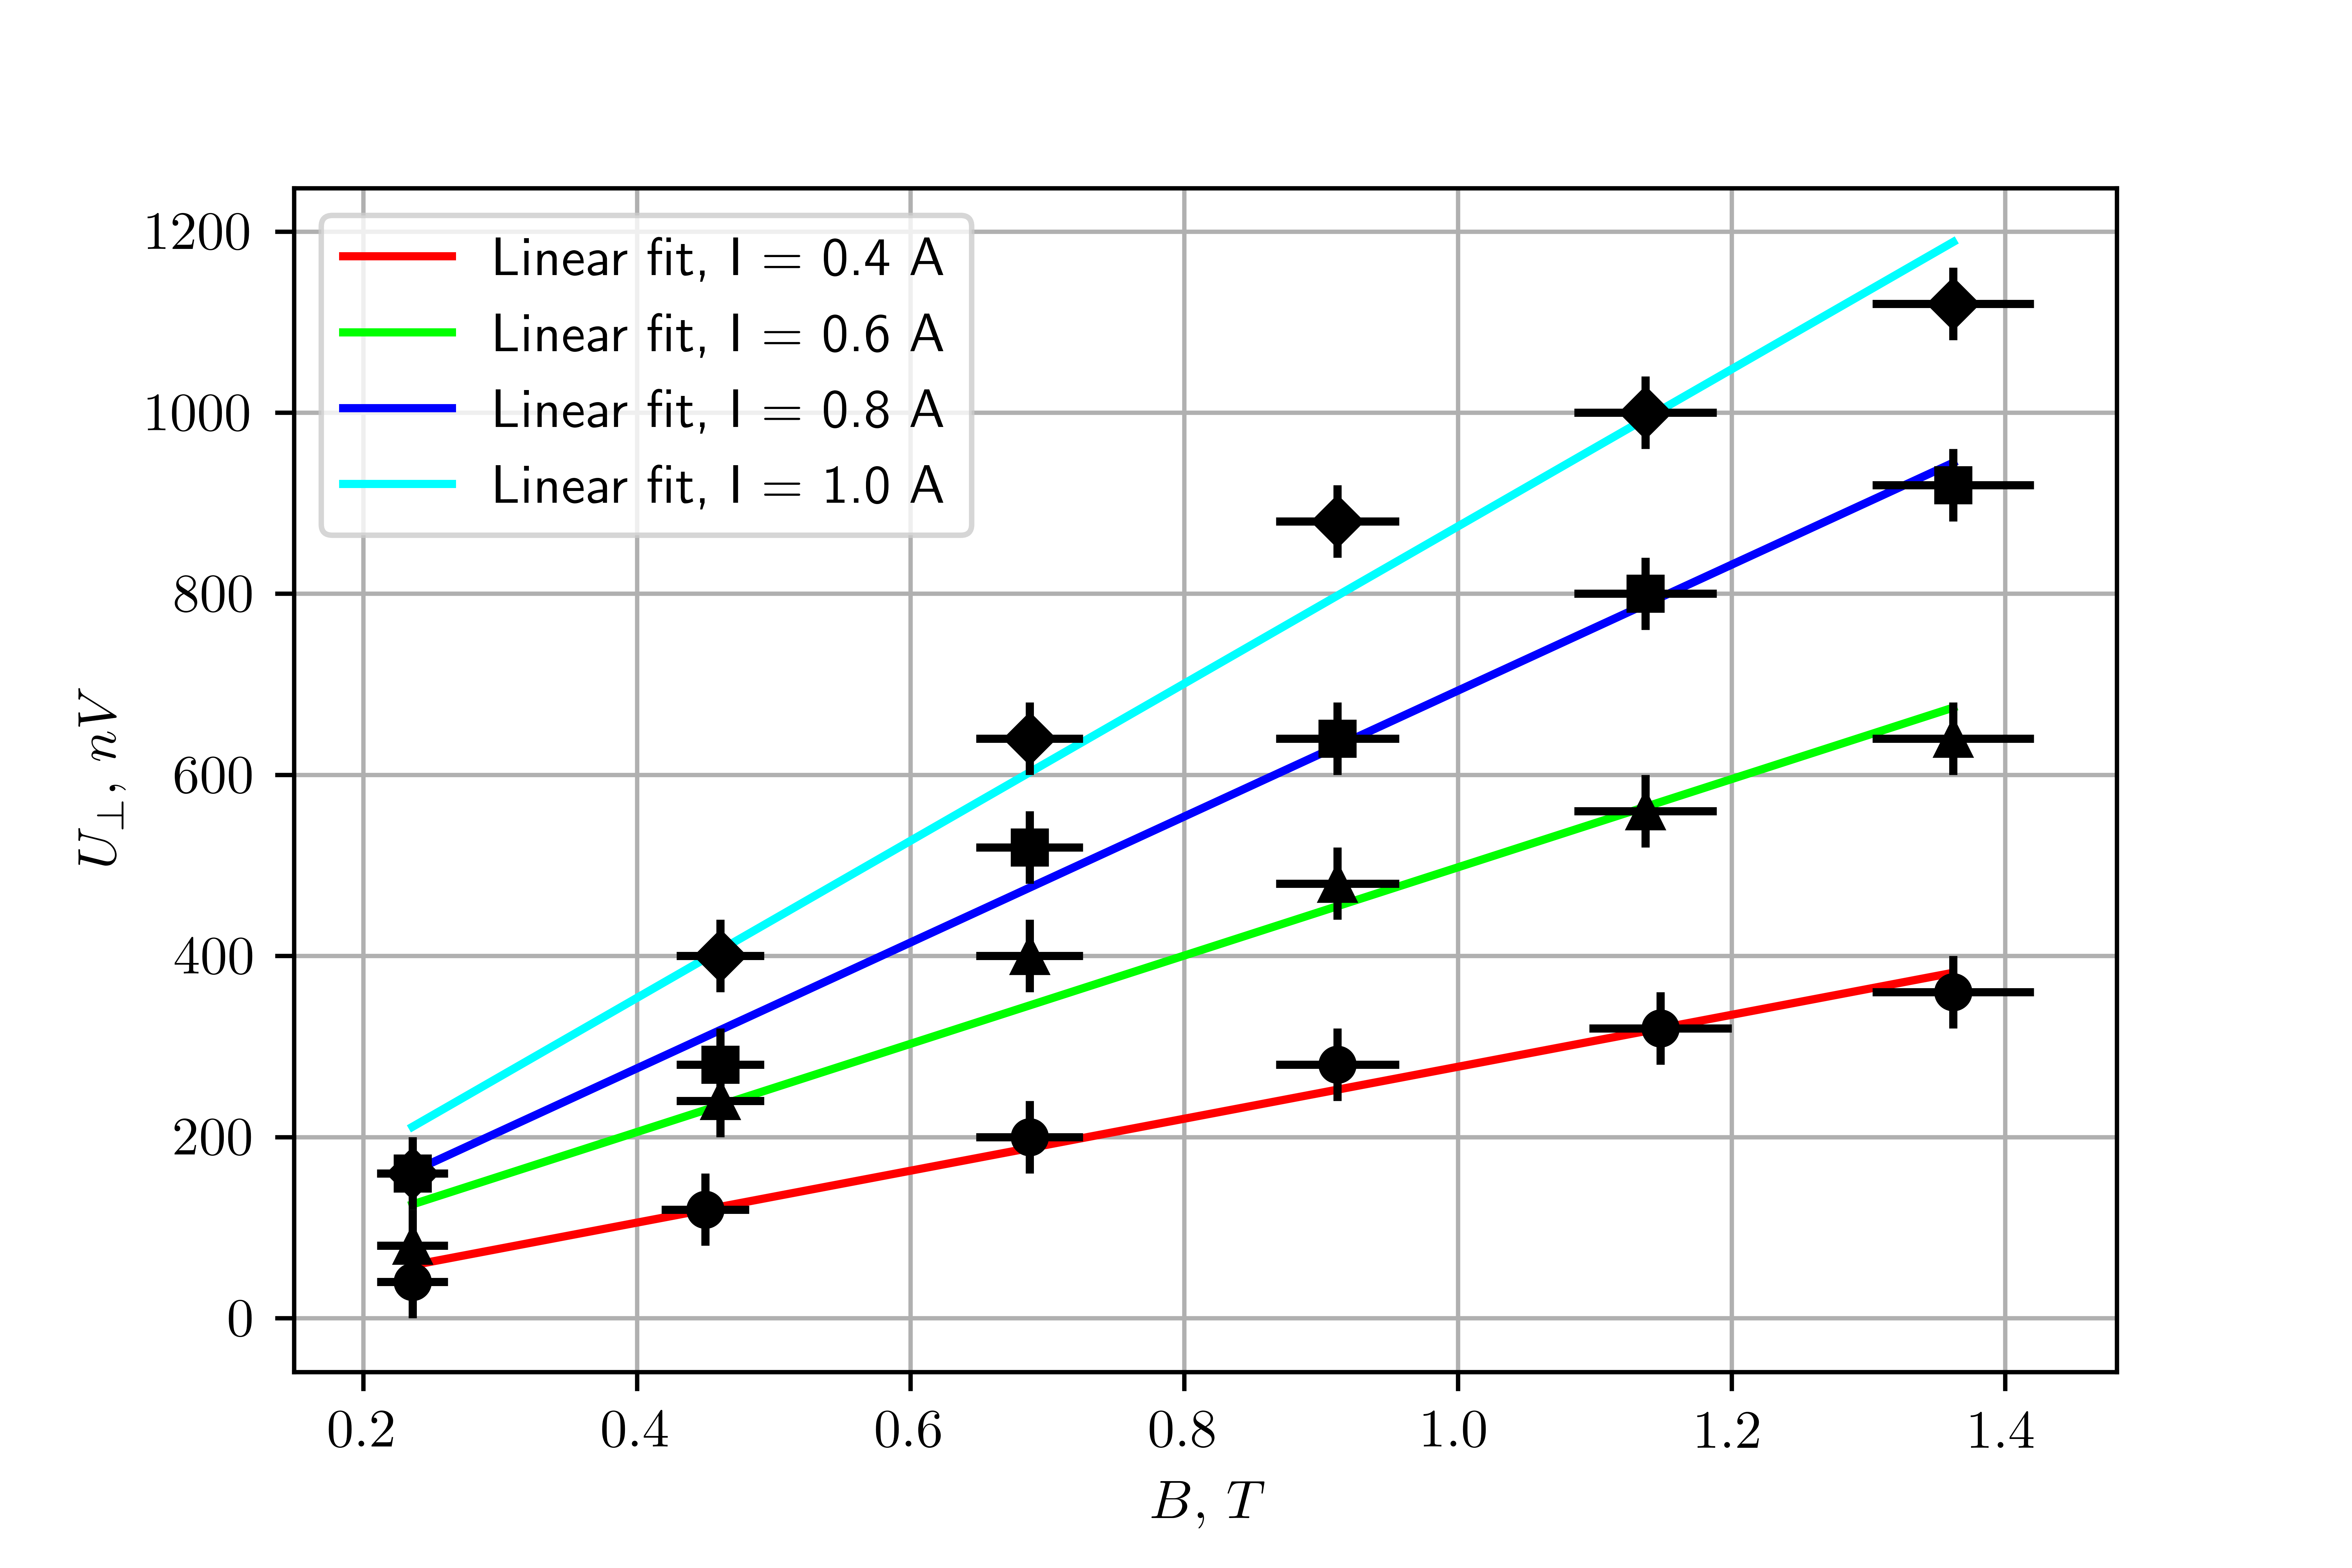
\includegraphics[scale=0.7]{PIC_5.png}
		\\\textbf{Рис. 5:} Графики $U_\perp(I)$ для меди
	\end{center}
	
	\begin{center}
		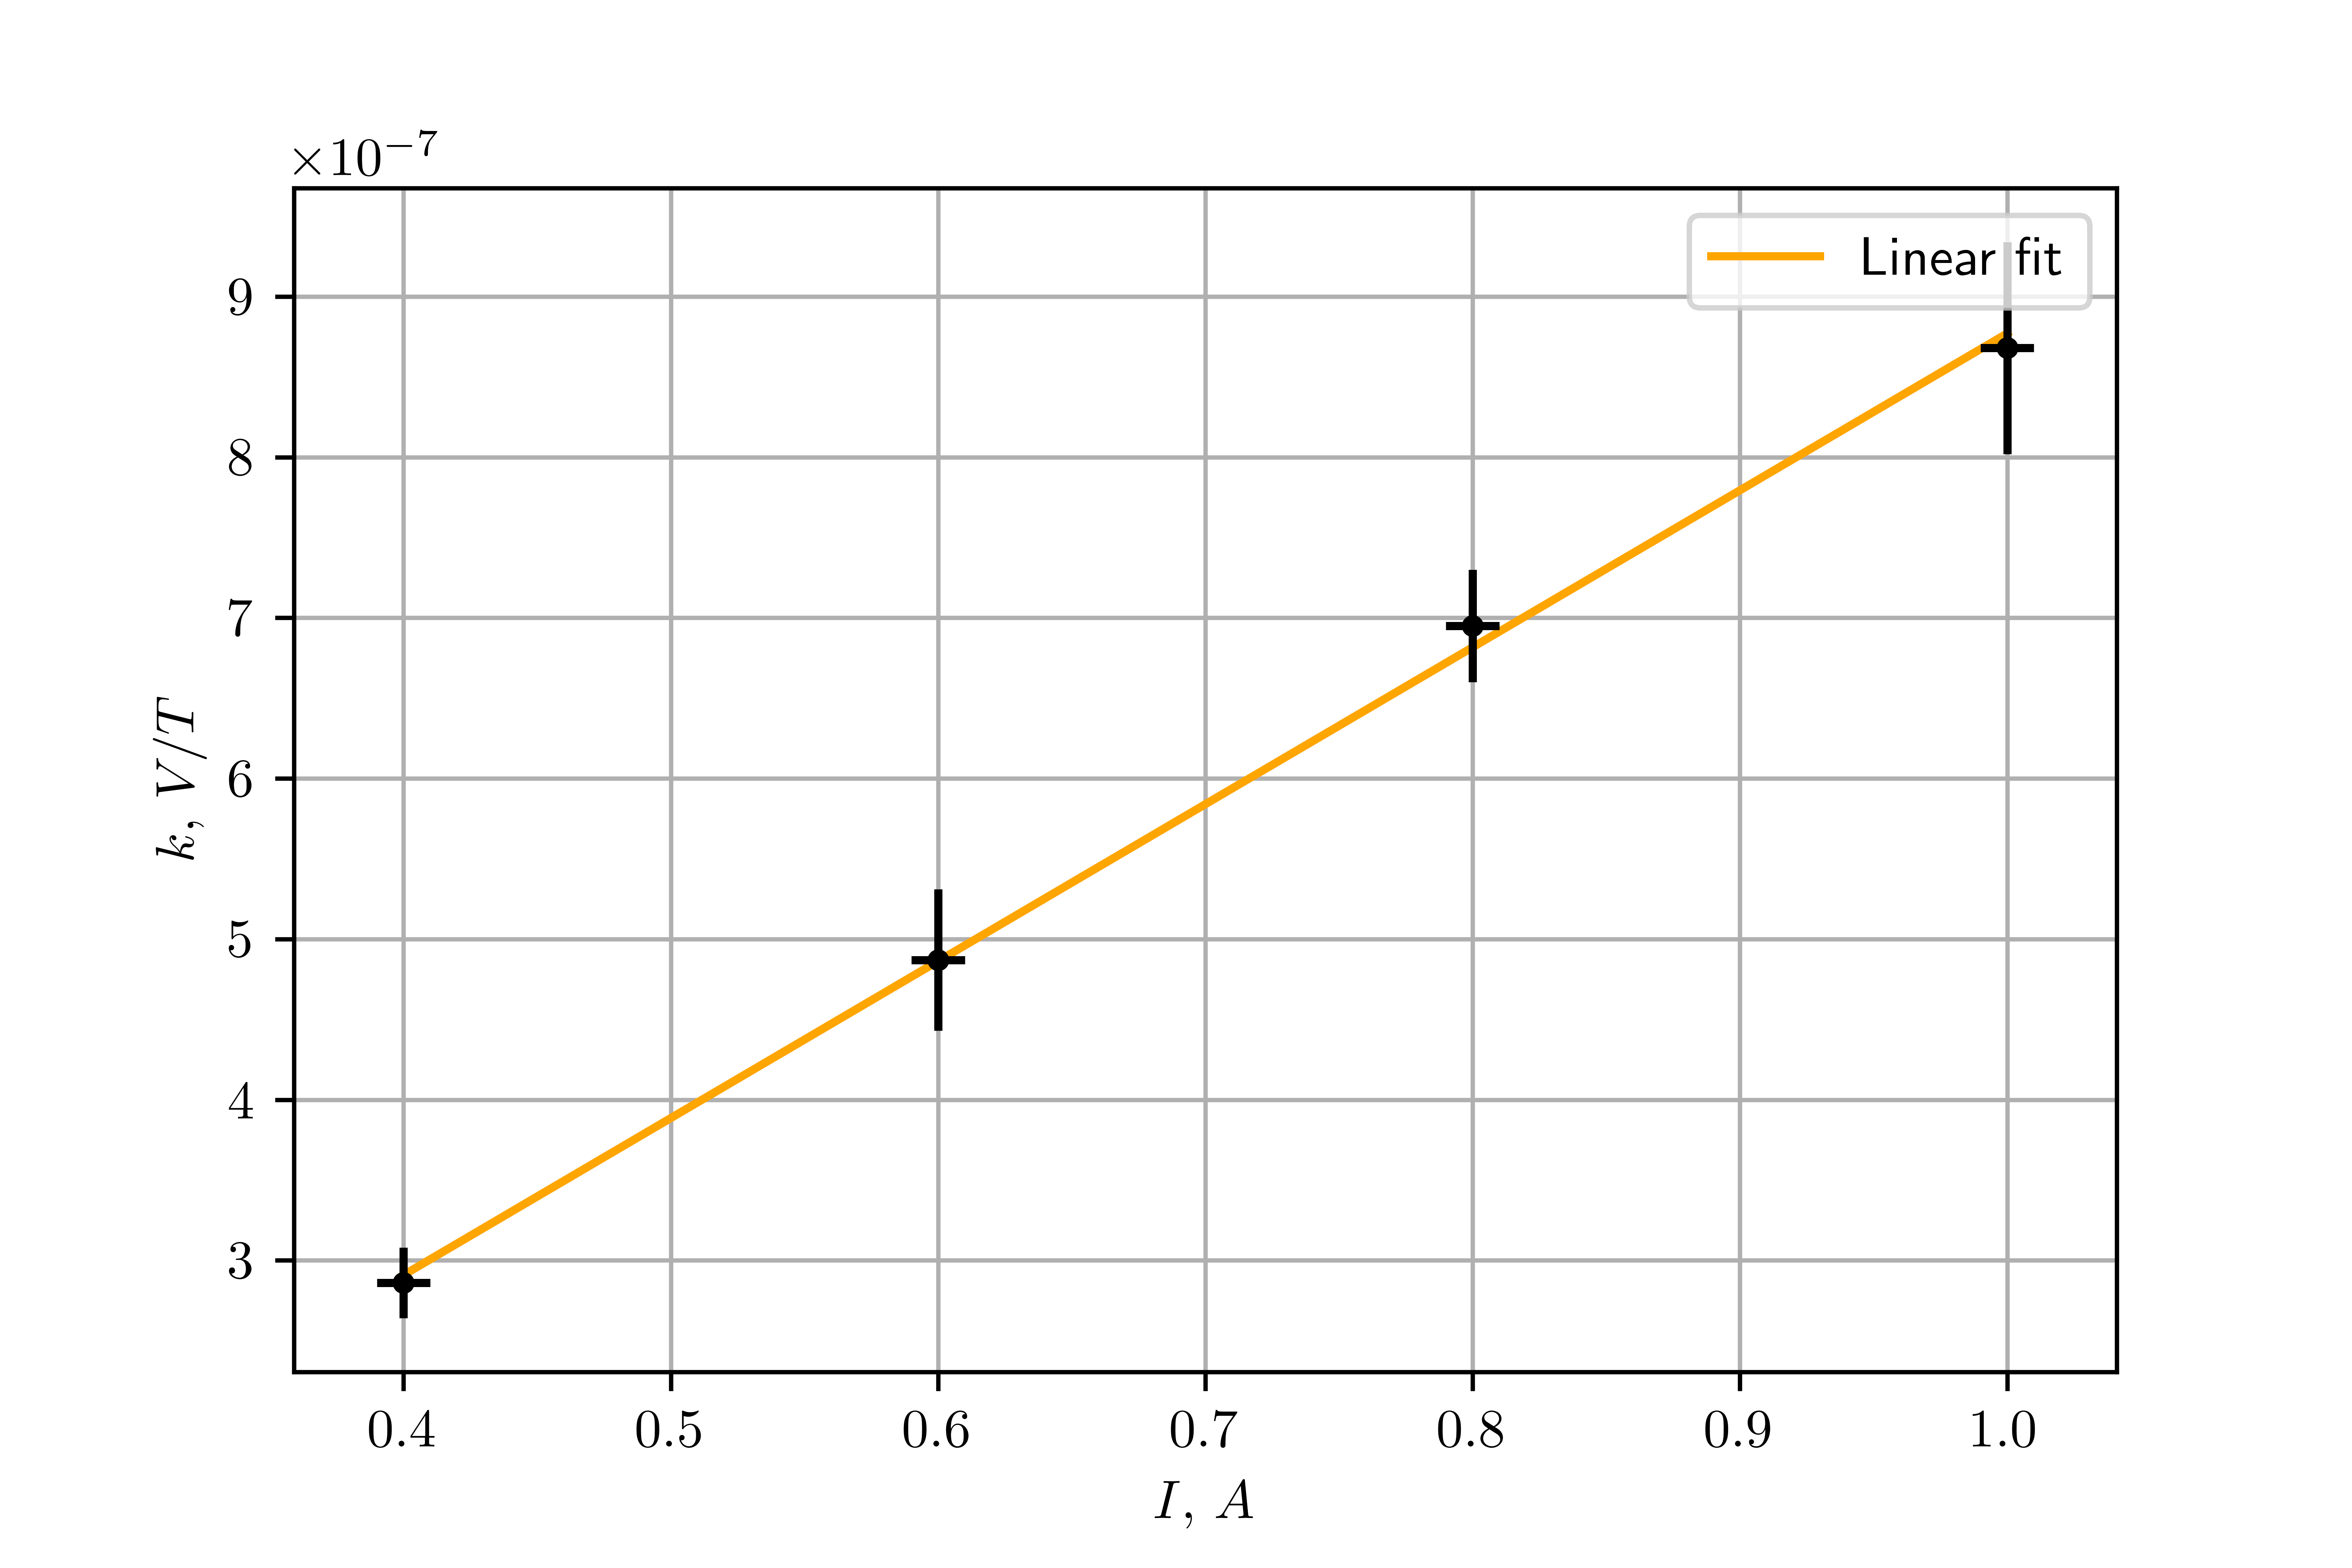
\includegraphics[scale=0.7]{PIC_6.png}
		\\\textbf{Рис. 6:} График $k(I)$ для меди
	\end{center}
	
	Наконец, методом линейной аппроксимации получаем:
	$$\gamma = (0.977 \pm 0.027) \cdot 10^{-6}\, \text{Ohm}/\text{T}$$
	
	Учитывая параметры образца $L_{34} = 6\, mm$, $l = 8\, mm$, $a = 0.05\, mm$, $U_{34} = 23 \mu V$:
	
	$$R_x = -\gamma a \approx -(4.9 \pm 0.2) \cdot 10^{-11}\, m^3/C$$
	
	Теперь рассчитаем концентрацию носителей проводимости, удельную проводимость и подвижность носителей:
	
	$$n = \sfrac{1}{R_xe} \approx -(0.12 \pm 0.01) \cdot 10^{30}\, 1/m^3$$
	
	$$\sigma = \sfrac{Il_{34}}{U_{34}al} \approx (0.63 \pm 0.06) \cdot 10^8\, 1/Ohm \cdot m$$
	
	$$b = R_x\sigma \approx (32 \pm 3)\, sm^2/V\cdot s$$
	 
	\newpage
	
	%Страница 7
	
	\begin{flushleft}
		\footnotesize{Эффект Холла в металлах} \hspace{\fill} \footnotesize{7}
		\\[-0.3cm]\noindent\rule{\textwidth}{0.3pt}
	\end{flushleft}	
	
	\paragraph{Исследование образца из цинка} \hfill
	
	Вначале по направлению ЭДС Холла определяем знак носителей проводимости -- -.

	\begin{center}
		\begin{tabular}{|c|c|c|c|}
			\hline
			\multicolumn{2}{|c|}{$I = (0.6 \pm 0.1)$ A} & \multicolumn{2}{|c|}{$U_0 = 10$ nV}
			\\\hline
			$I_m$, A & $B$, T & $U_{24}$, un & $U_\perp$, nV
			\\\hline
			$0.20 \pm 0.01$ & $0.236 \pm 0.026$ & $16.0 \pm 0.5$ & $240 \pm 40$
			\\\hline
			$0.40 \pm 0.01$ & $0.461 \pm 0.032$ & $22.0 \pm 0.5$ & $480 \pm 40$
			\\\hline
			$0.60 \pm 0.01$ & $0.687 \pm 0.039$ & $27.0 \pm 0.5$ & $680 \pm 40$
			\\\hline
			$0.80 \pm 0.01$ & $0.912 \pm 0.045$ & $30.0 \pm 0.5$ & $800 \pm 40$
			\\\hline
			$1.00 \pm 0.01$ & $1.137 \pm 0.052$ & $33.0 \pm 0.5$ & $920 \pm 40$
			\\\hline
			$1.20 \pm 0.01$ & $1.362 \pm 0.059$ & $36.0 \pm 0.5$ & $1040 \pm 40$
			\\\hline
		\end{tabular}	
		\\\textbf{Табл. 4:} Исследование образца из цинка
	\end{center}	
	
	\begin{center}
		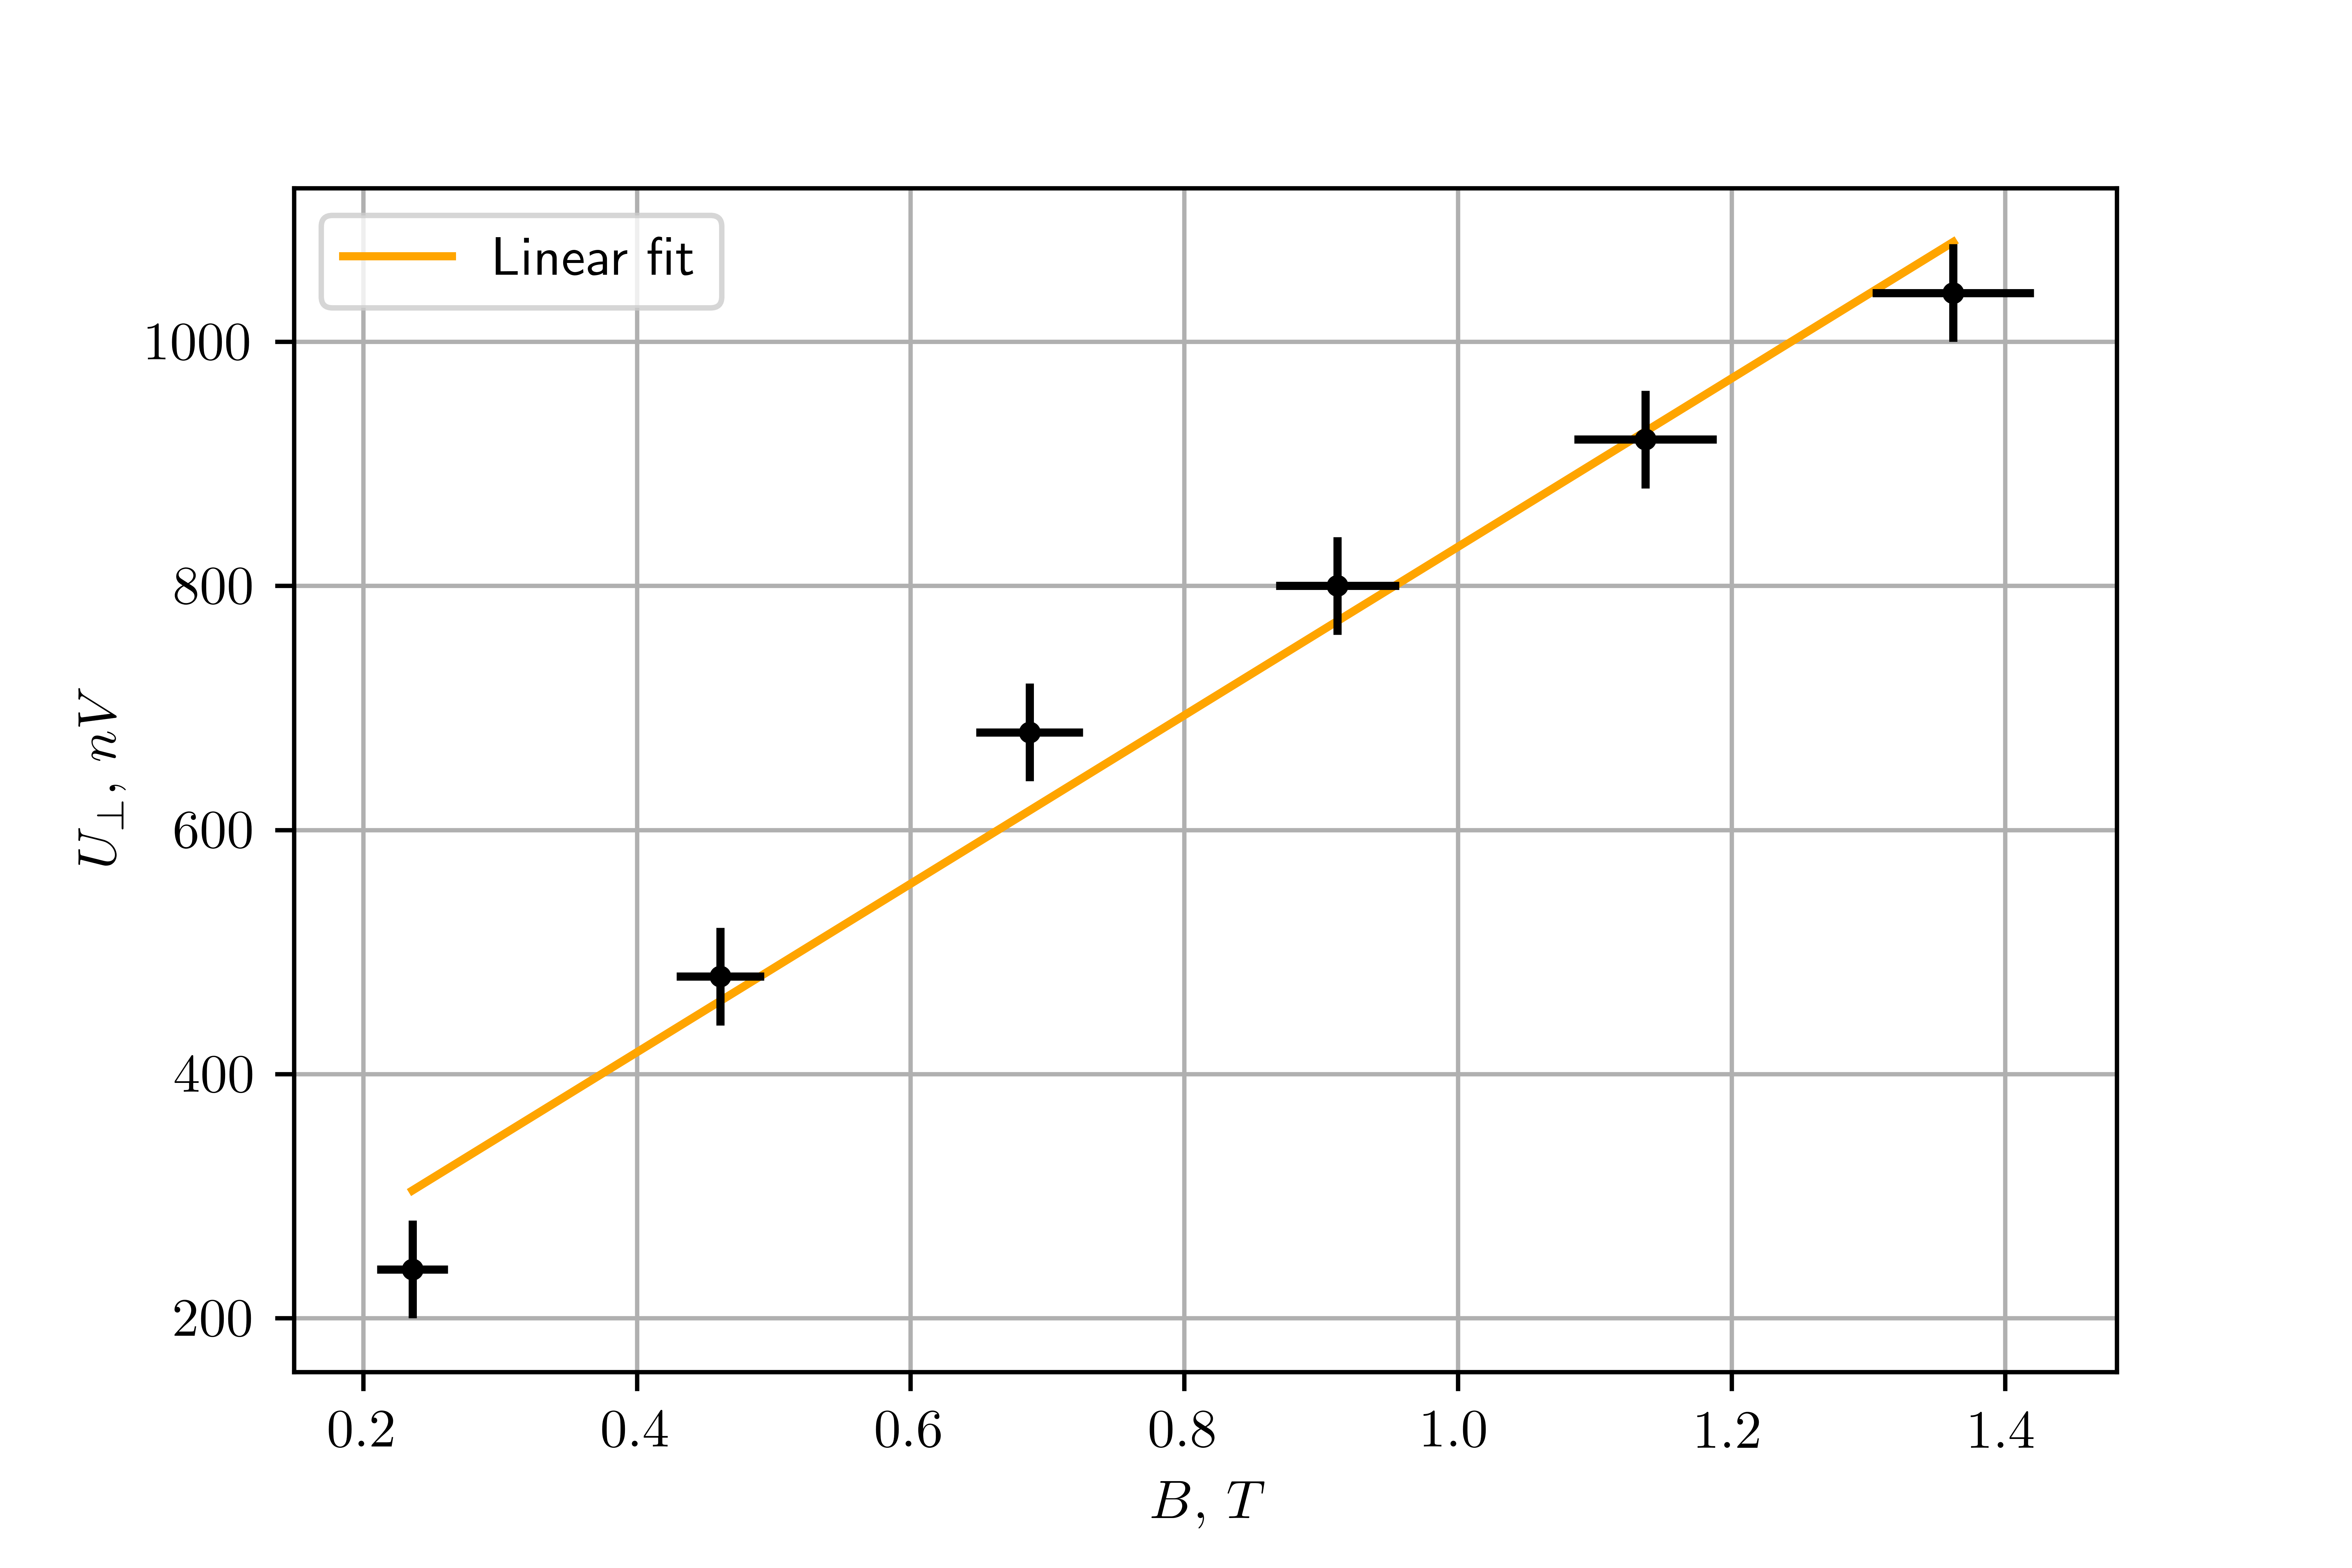
\includegraphics[scale=0.7]{PIC_7.png}
		\\\textbf{Рис. 7:} График $U_\perp(I)$ для цинка
	\end{center}
	
	Методом линейной аппроксимации получаем:
	
	$$k = (6.90 \pm 0.56) \cdot 10^{-7}\, V/T$$
	
	Учитывая параметры образца $L_{34} = 4\, mm$, $l = 10\, mm$, $a = 0.08\, mm$, $U_{34} = 26 \mu V$:

	$$R_x = \sfrac{Ba}{I} \approx (9.5 \pm 0.9) \cdot 10^{-11} m^3/C$$
	
	Теперь рассчитаем концентрацию носителей проводимости, удельную проводимость и подвижность носителей:
	
	$$n = \sfrac{1}{R_xe} \approx (0.60 \pm 0.06) \cdot 10^{30}\, 1/m^3$$
	
	$$\sigma = \sfrac{Il_{34}}{U_{34}al} \approx (0.19 \pm 0.02) \cdot 10^8\, 1/Ohm \cdot m$$
	
	$$b = R_x\sigma \approx (18 \pm 2)\, sm^2/V\cdot s$$
	
	\section{Выводы}
	
	Проведено исследование эффекта Холла на проводниках из меди и цинка. В результате работы определены знаки носителей проводимости (+ для меди и - для цинка), а также некоторые постоянные:
	
	Постоянные Холла:
	
	$$R_{x, Cu} = -(4.9 \pm 0.2) \cdot 10^{-11}\, m^3/C\ \ \ \ \ \ \ \ R_{x, Zn} = (9.5 \pm 0.9) \cdot 10^{-11} m^3/C$$
	
	В сравнении с табличными значениями:
	
	$$R_{x, Cu} = -5.3 \cdot 10^{-11}\, m^3/C\ \ \ \ \ \ \ \ R_{x, Zn} = 10.4 \cdot 10^{-11} m^3/C$$
	
	Концентрации носителей проводимости:
		
	$$n_{Cu} = -(0.12 \pm 0.01) \cdot 10^{30}\, 1/m^3\ \ \ \ \ \ \ \ n_{Zn} = (0.60 \pm 0.006) \cdot 10^{30} 1/m^3$$
	
	Удельные проводимости:
	
		$$\sigma_{Cu} = (0.63 \pm 0.06) \cdot 10^{8}\, 1/Ohm \cdot m\ \ \ \ \ \ \ \ \sigma_{Zn} = (0.19 \pm 0.02) \cdot 10^{8} /Ohm \cdot m$$	
	
	В сравнении с табличными значениями:
	
	$$\sigma_{Cu} = 0.56 \cdot 10^{8}\, 1/Ohm \cdot m\ \ \ \ \ \ \ \ \sigma_{Zn} = 0.16 \cdot 10^{8} /Ohm \cdot m$$	
	
	Подвижности носителей:
	
	$$b_{Cu} = (32 \pm 3) \, sm^2/V \cdot s\ \ \ \ \ \ \ \ b_{Zn} = (18 \pm 2) sm^2/V \cdot s$$
	
	В сравнении с табличными значениями:

	$$b_{Cu} = 32 \, sm^2/V \cdot s\ \ \ \ \ \ \ \ b_{Zn} = 17.5 sm^2/V \cdot s$$


\end{document}